\documentclass{beamer}
\usepackage[galician]{babel}
\usepackage[utf8]{inputenc}
\usetheme{Madrid}
%\usecolortheme{beaver}

\usepackage{outlines}
\usepackage{wrapfig}
%Título

\title{First Task: VELO Tracks}
\author{Adrián Casais Vidal}
\institute[USC]{Universidade de Santiago de Compostela}
\date{\today}

\begin{document}
%%Introducción
\begin{frame}
\titlepage
\end{frame}
\begin{frame}
\frametitle{Track Matching}
Definition of kinematical variables:
\begin{align}
R &= \sqrt{\phi^2+\eta^2}\\ 
Z &= \text{distance from PV}
\end{align}
\begin{itemize}
\item $\Delta$R $<$ 0.5 
\item $\Delta$Z $<$ 100 mm
\item Particle-Track matching was performed with this criteria
\item The data was stored in the corresponding ROOT files for further \textit{analysis}.
\item It was found that, of all tracks matched, the 37.99 \% of them corresponds to VELO tracks, applying this criteria.  
\end{itemize}
\end{frame}
\begin{frame}
\frametitle{Matching VELO tracks to Long tracks}

Some VELO tracks could have been mismatched also as long tracks and for that reason a matching procedure involving a similar approach was performed, this time the cut value is chosen as $\Delta R$ = 0.3.  
\end{frame}
\begin{frame}
\frametitle{Distribution of ID's}
\begin{centering}
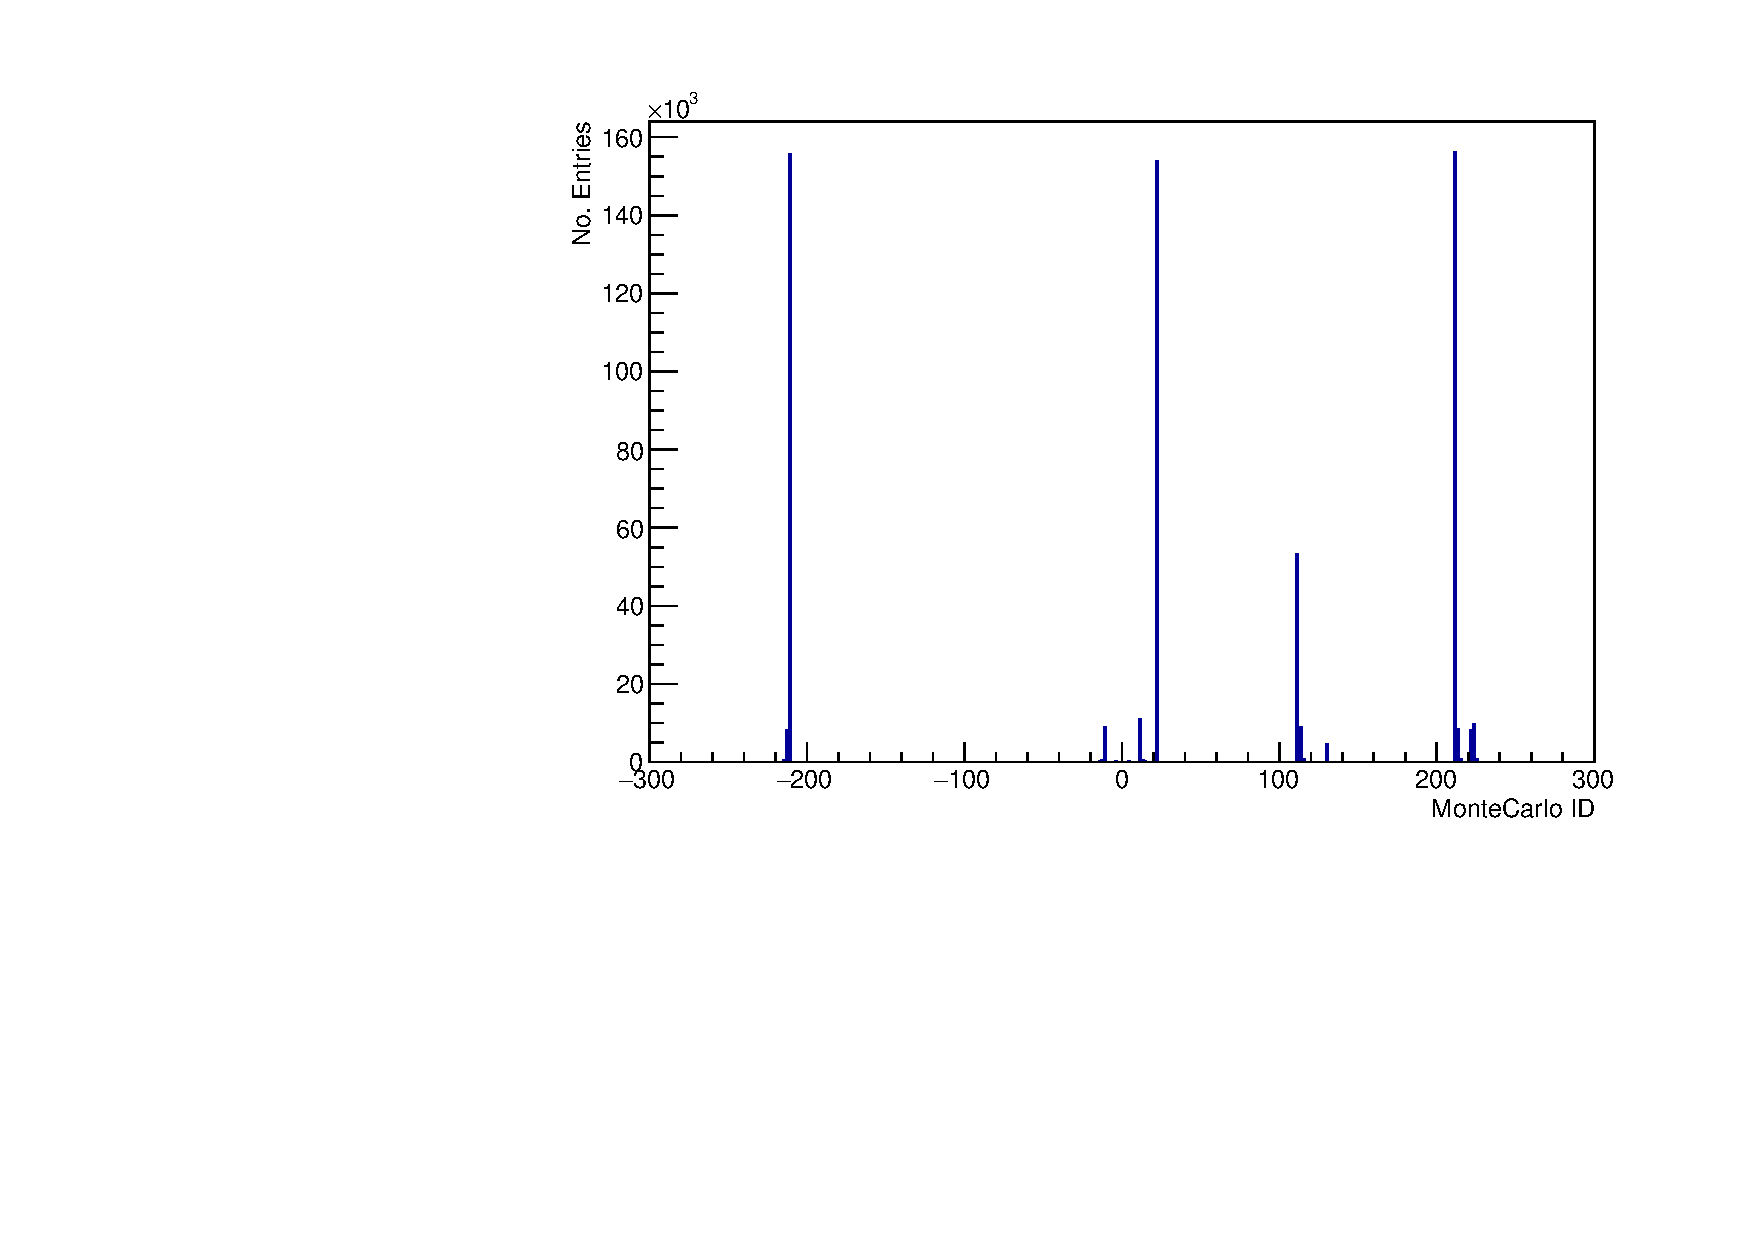
\includegraphics[width=0.8\textwidth]{MC_ID.pdf}
\end{centering}
\end{frame}

\begin{frame}
\frametitle{Distribution of ID's}
\begin{itemize}
\item 84 \% of events in the range [-300,300], if we extend the range to [-2212,2212], 96 \% of the events are contained there. 
\item 21.88 \% of $\gamma$'s.
\item 44.46\% of $\pi^{\pm}$
\item 1.57\% of e$^{-}$
\item 1.26\% of e$^{+}$ (different eff ?)
\item 0.64\% of K$^0_S$
\item 1.64\% of p
\item 1.37\% of p$^{-}$
\item 0.64\% of n
\end{itemize}
\end{frame}

\begin{frame}
\frametitle{Distribution of Momentum}
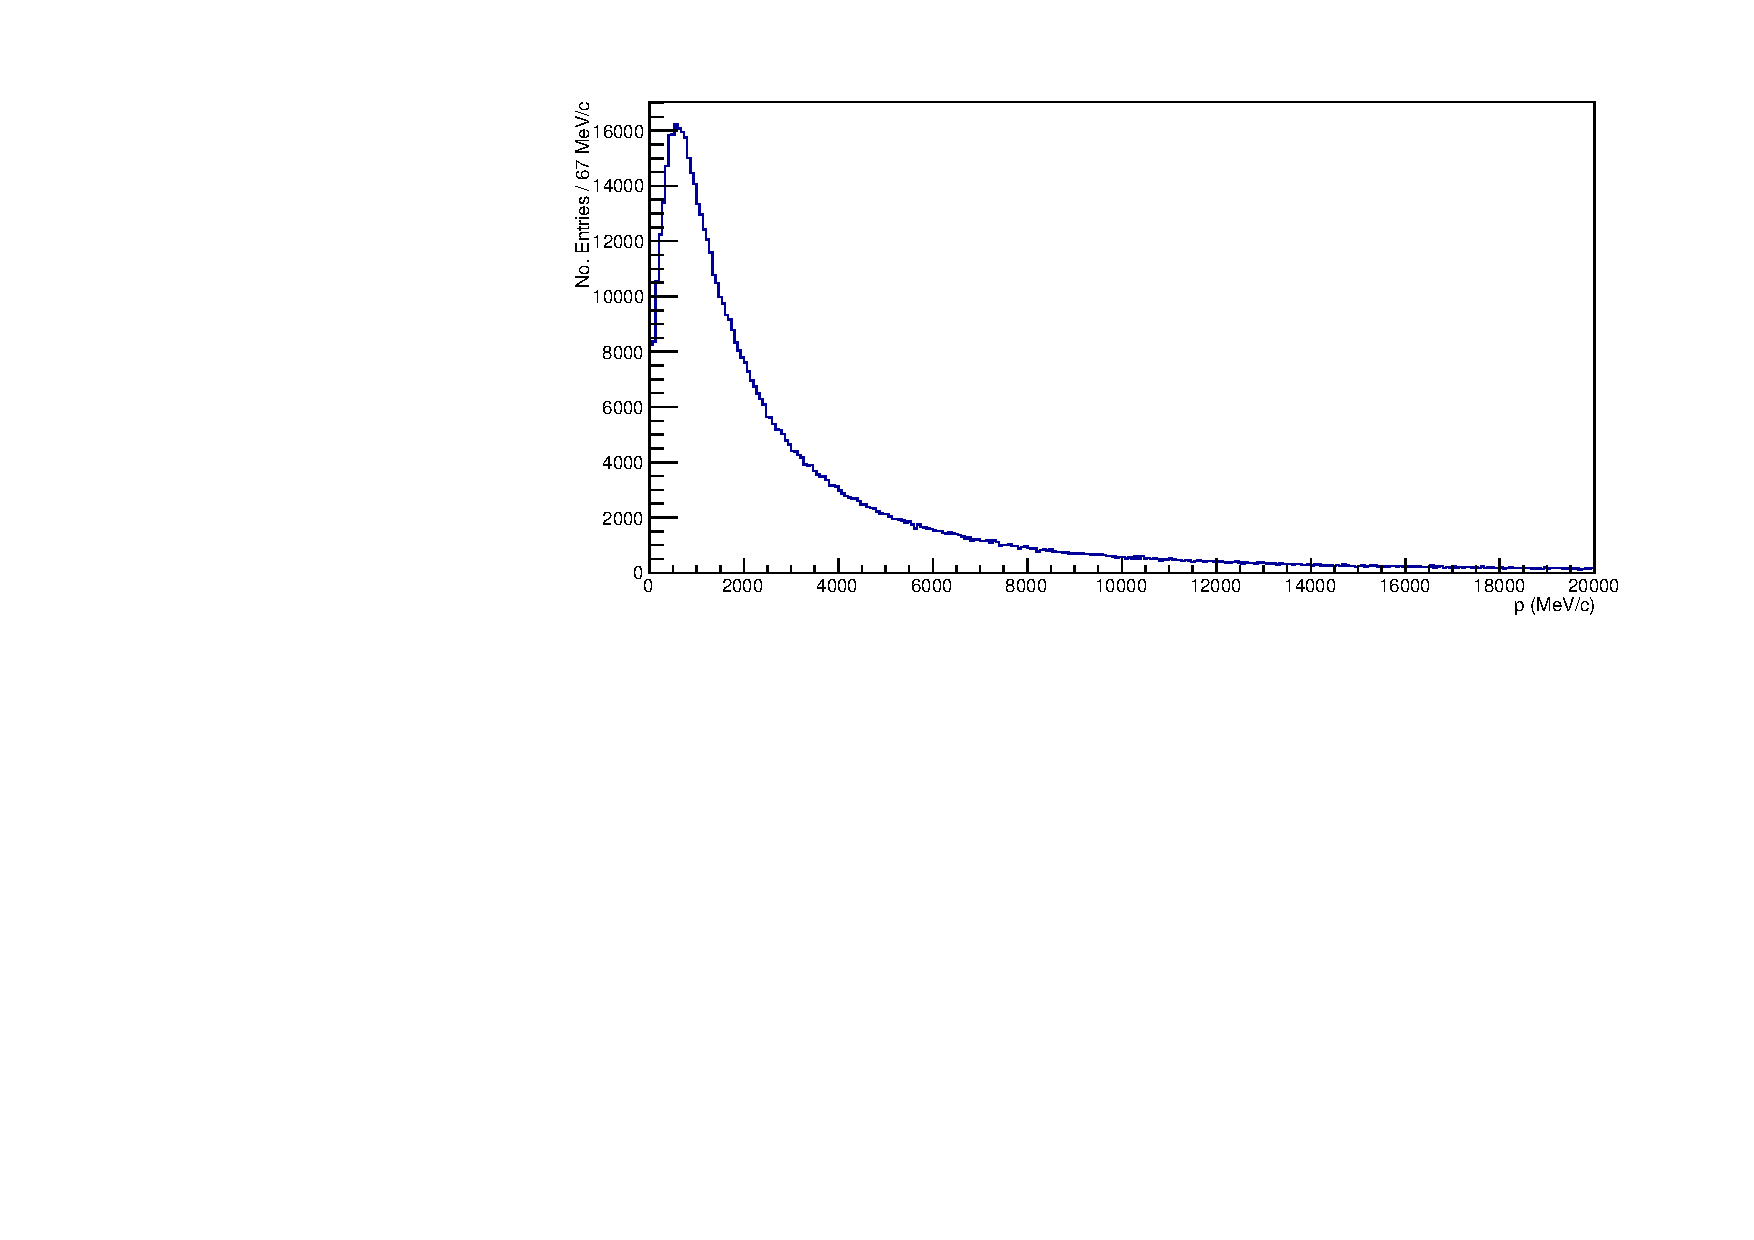
\includegraphics[width=0.8\textwidth]{p.pdf}
\end{frame}

\begin{frame}
\frametitle{Distribution of $\eta$}
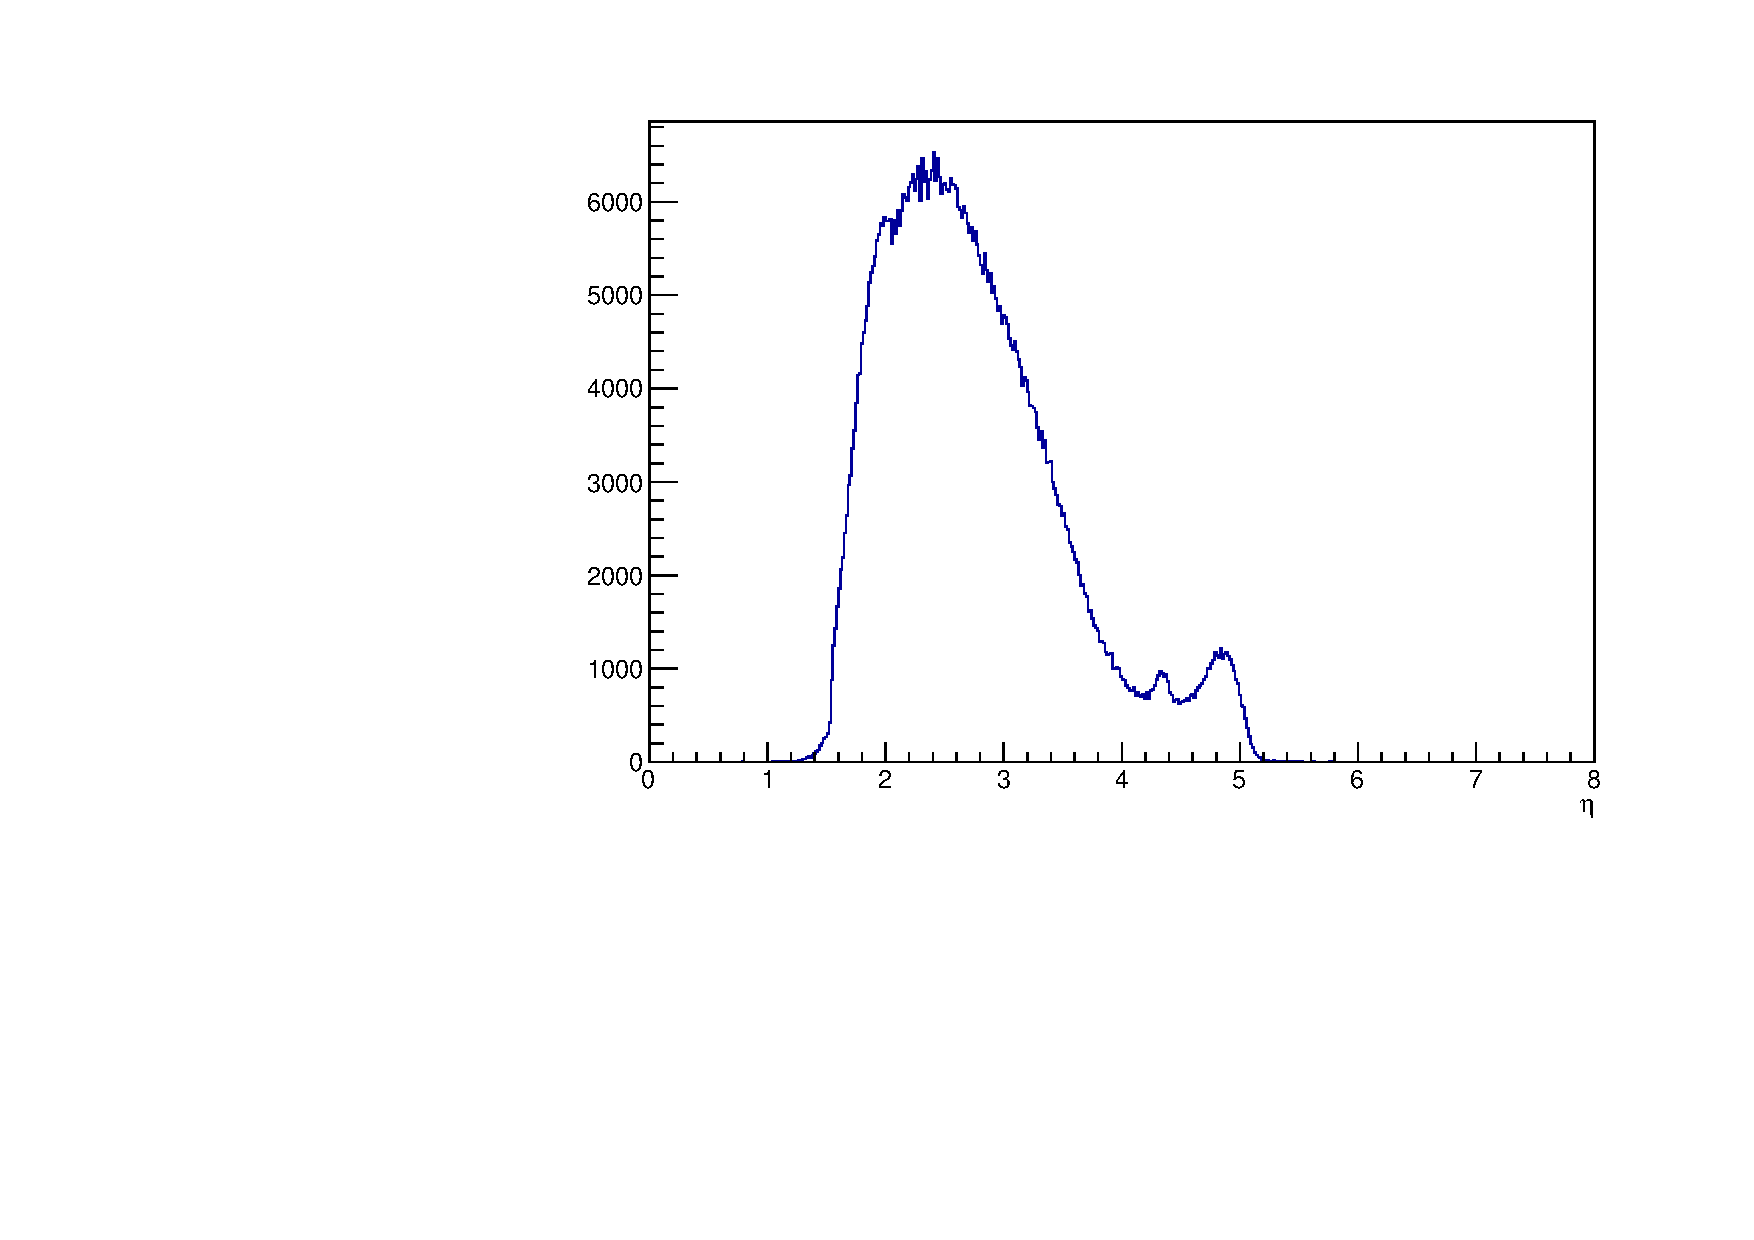
\includegraphics[width=0.8\textwidth]{eta.pdf}
\end{frame}


\begin{frame}
\frametitle{Distribution of $\phi$}
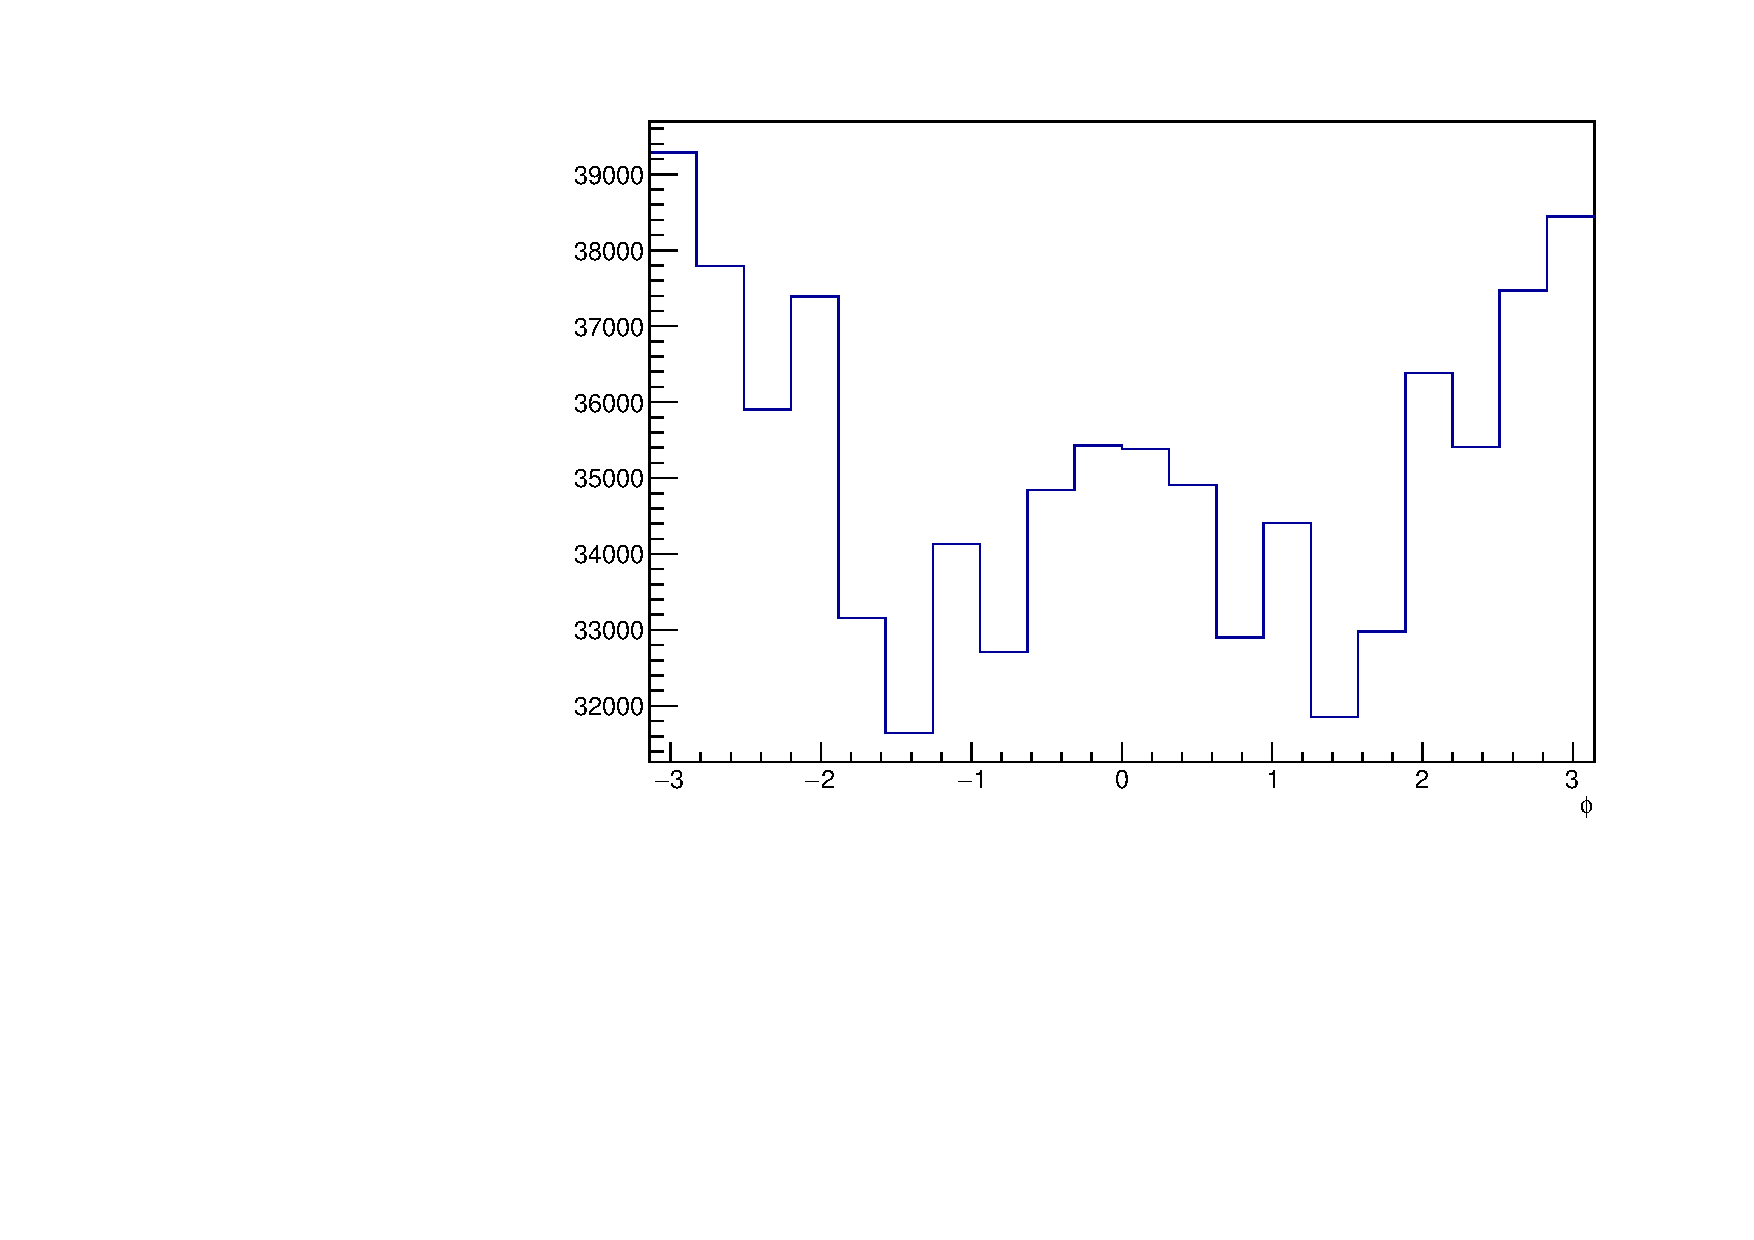
\includegraphics[width=0.8\textwidth]{phi.pdf}
\end{frame}

\begin{frame}
\frametitle{Exclusion of ghosts}
Now the same distributions will be shown excluding those MCParticles whose associated VELO track is matched to a LONG track.  
\end{frame}

\begin{frame}
\frametitle{Distribution of Momentum}
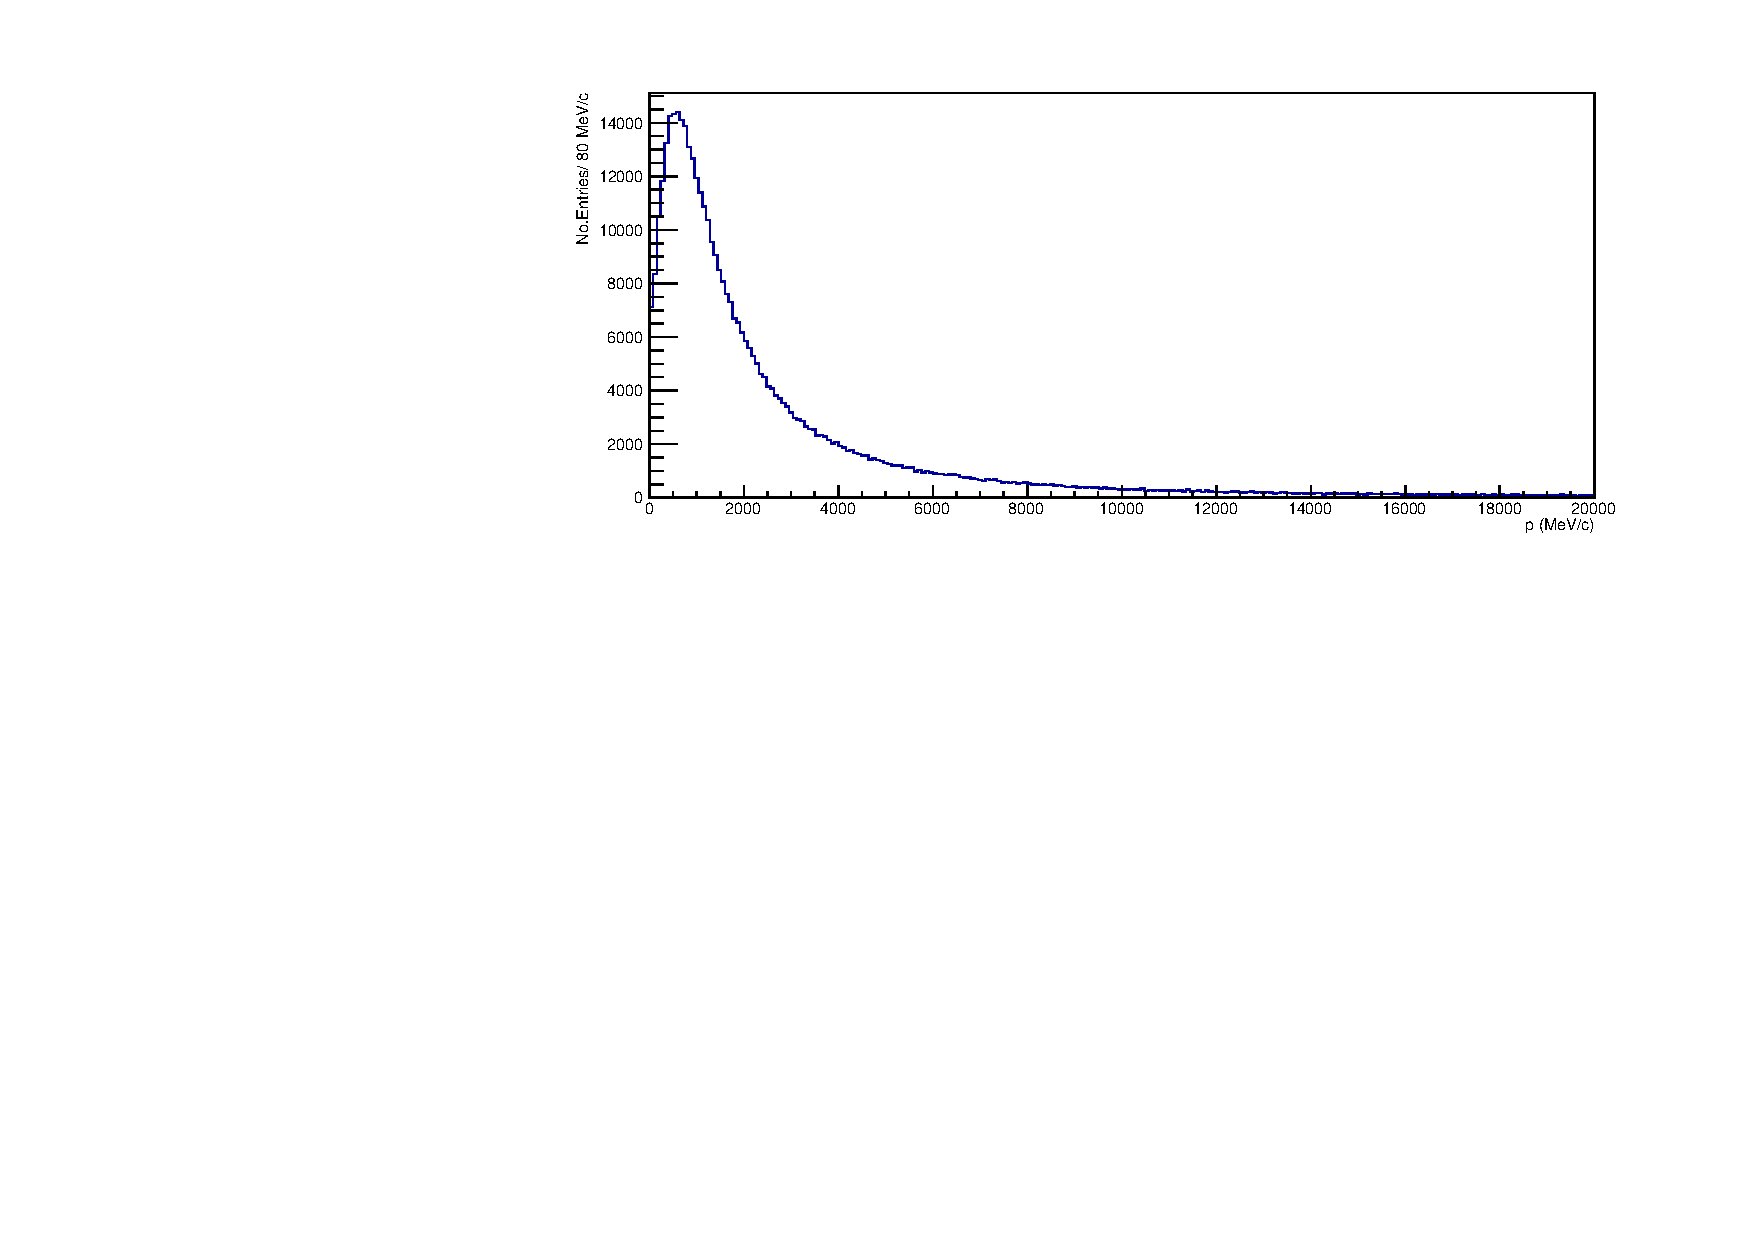
\includegraphics[width=\textwidth]{pwoghosts.pdf}
\end{frame}

\begin{frame}
\frametitle{Distribution of $\eta$}
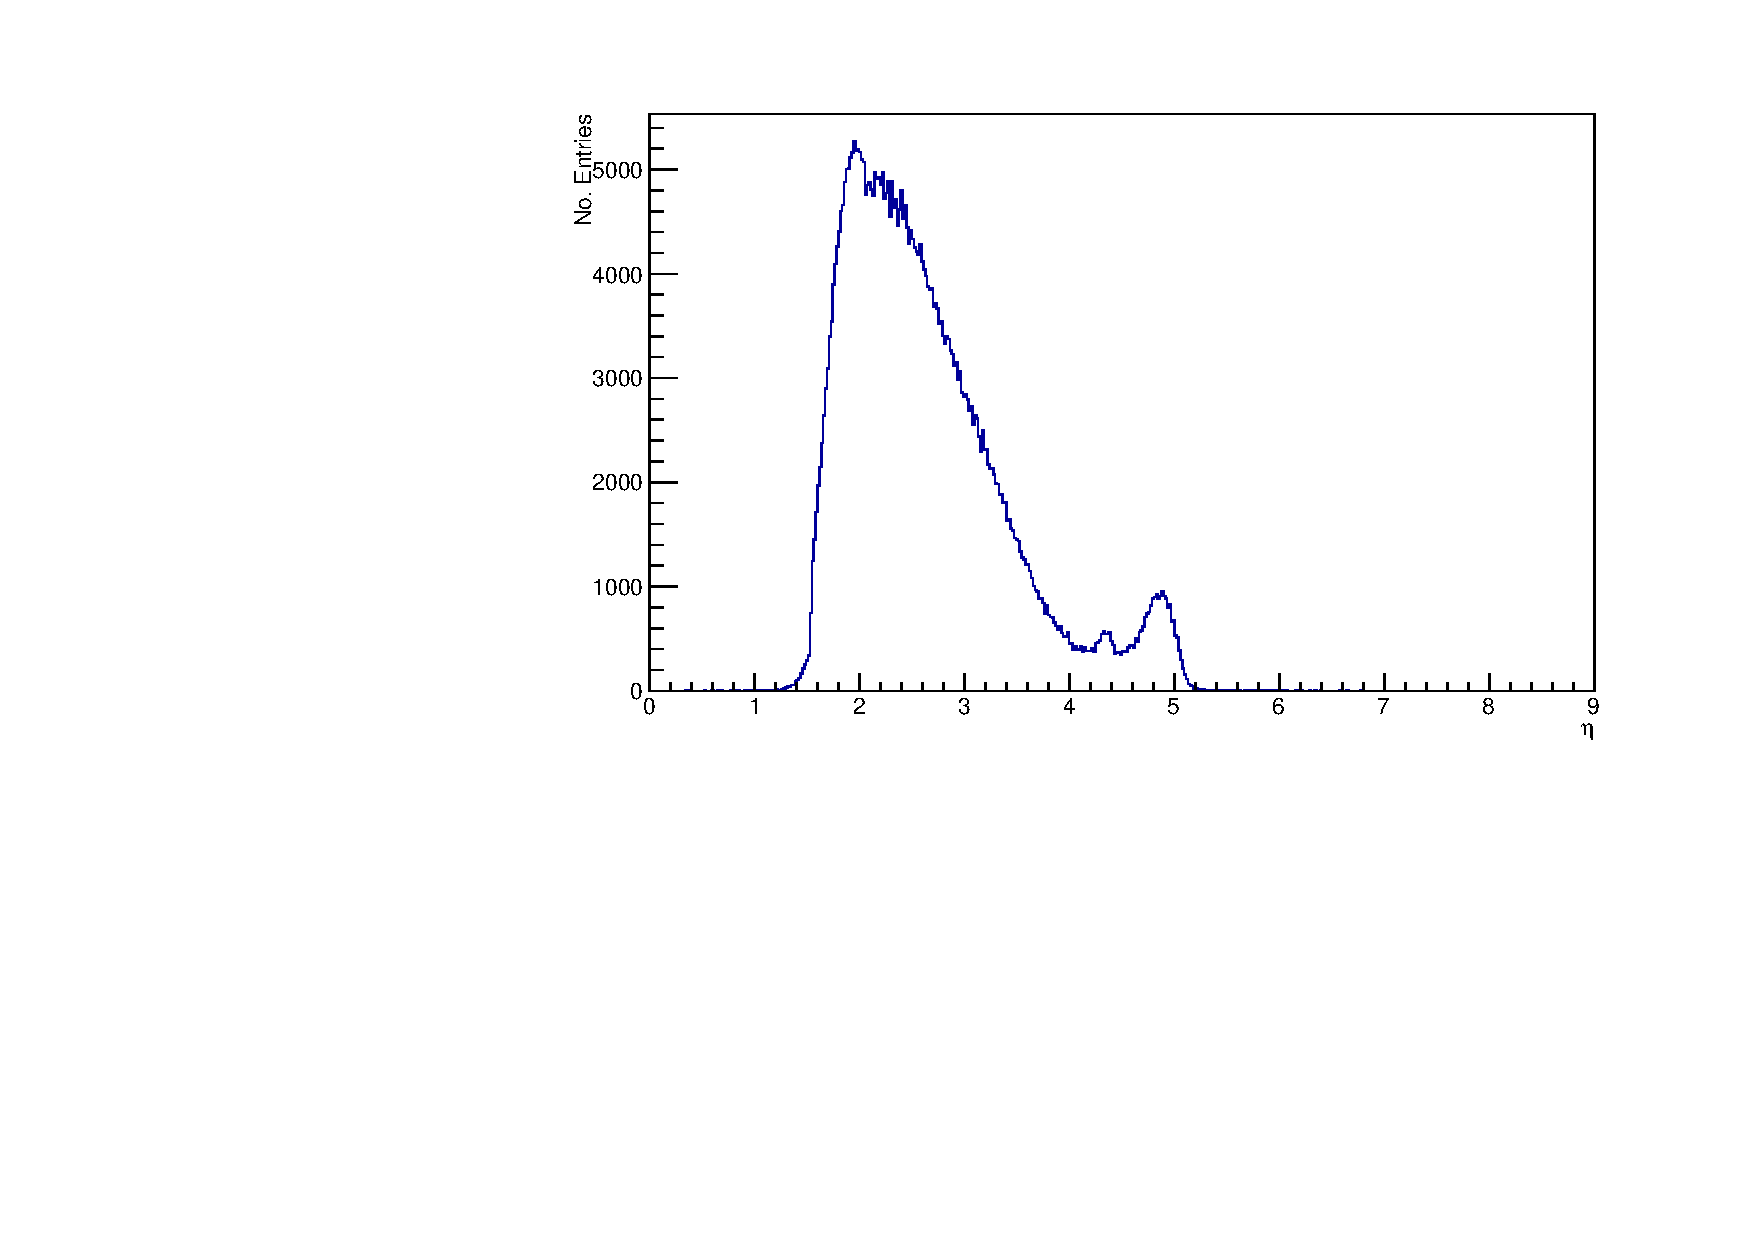
\includegraphics[width=0.8\textwidth]{etawoghosts.pdf}
\end{frame}


\begin{frame}
\frametitle{Distribution of $\phi$}
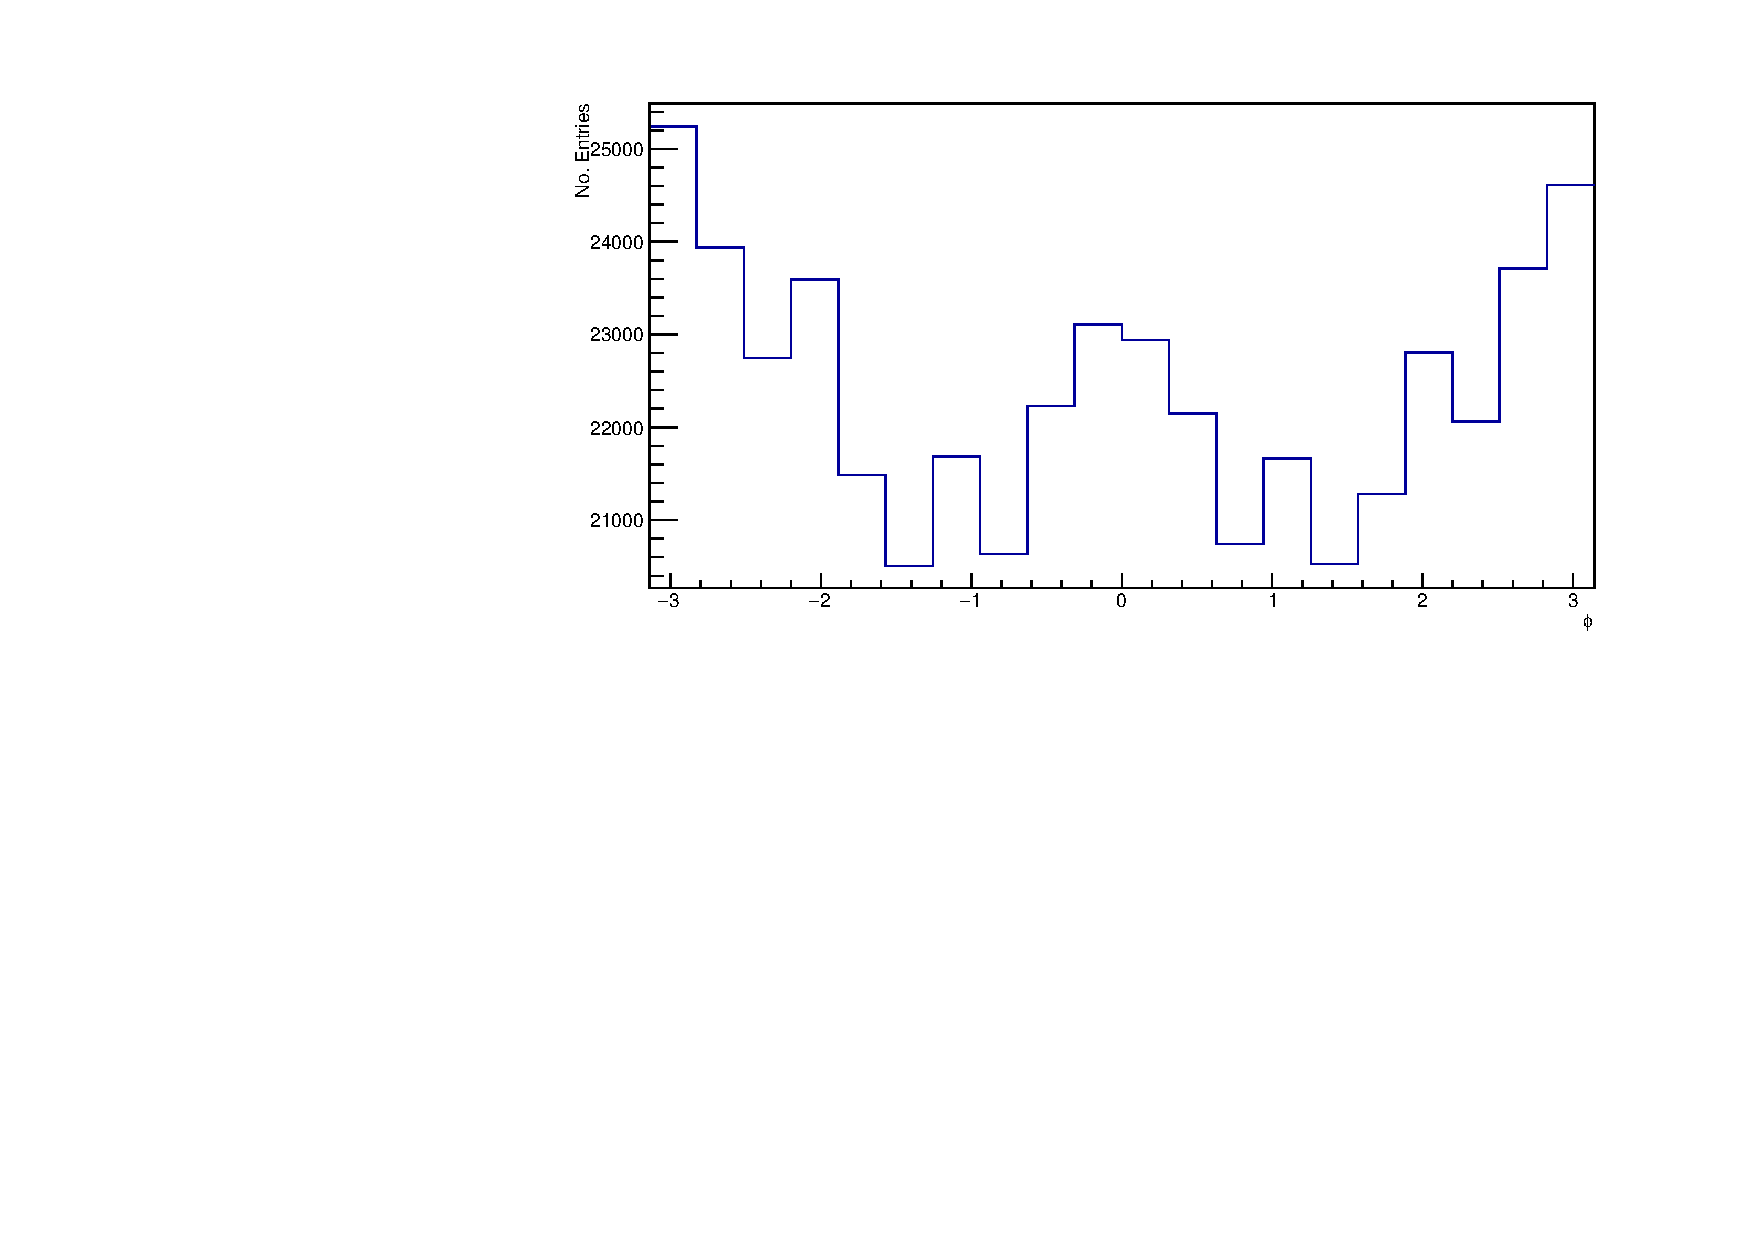
\includegraphics[width=0.8\textwidth]{phiwoghosts.pdf}
\end{frame}

\begin{frame}
\frametitle{$\Delta R$ Background}
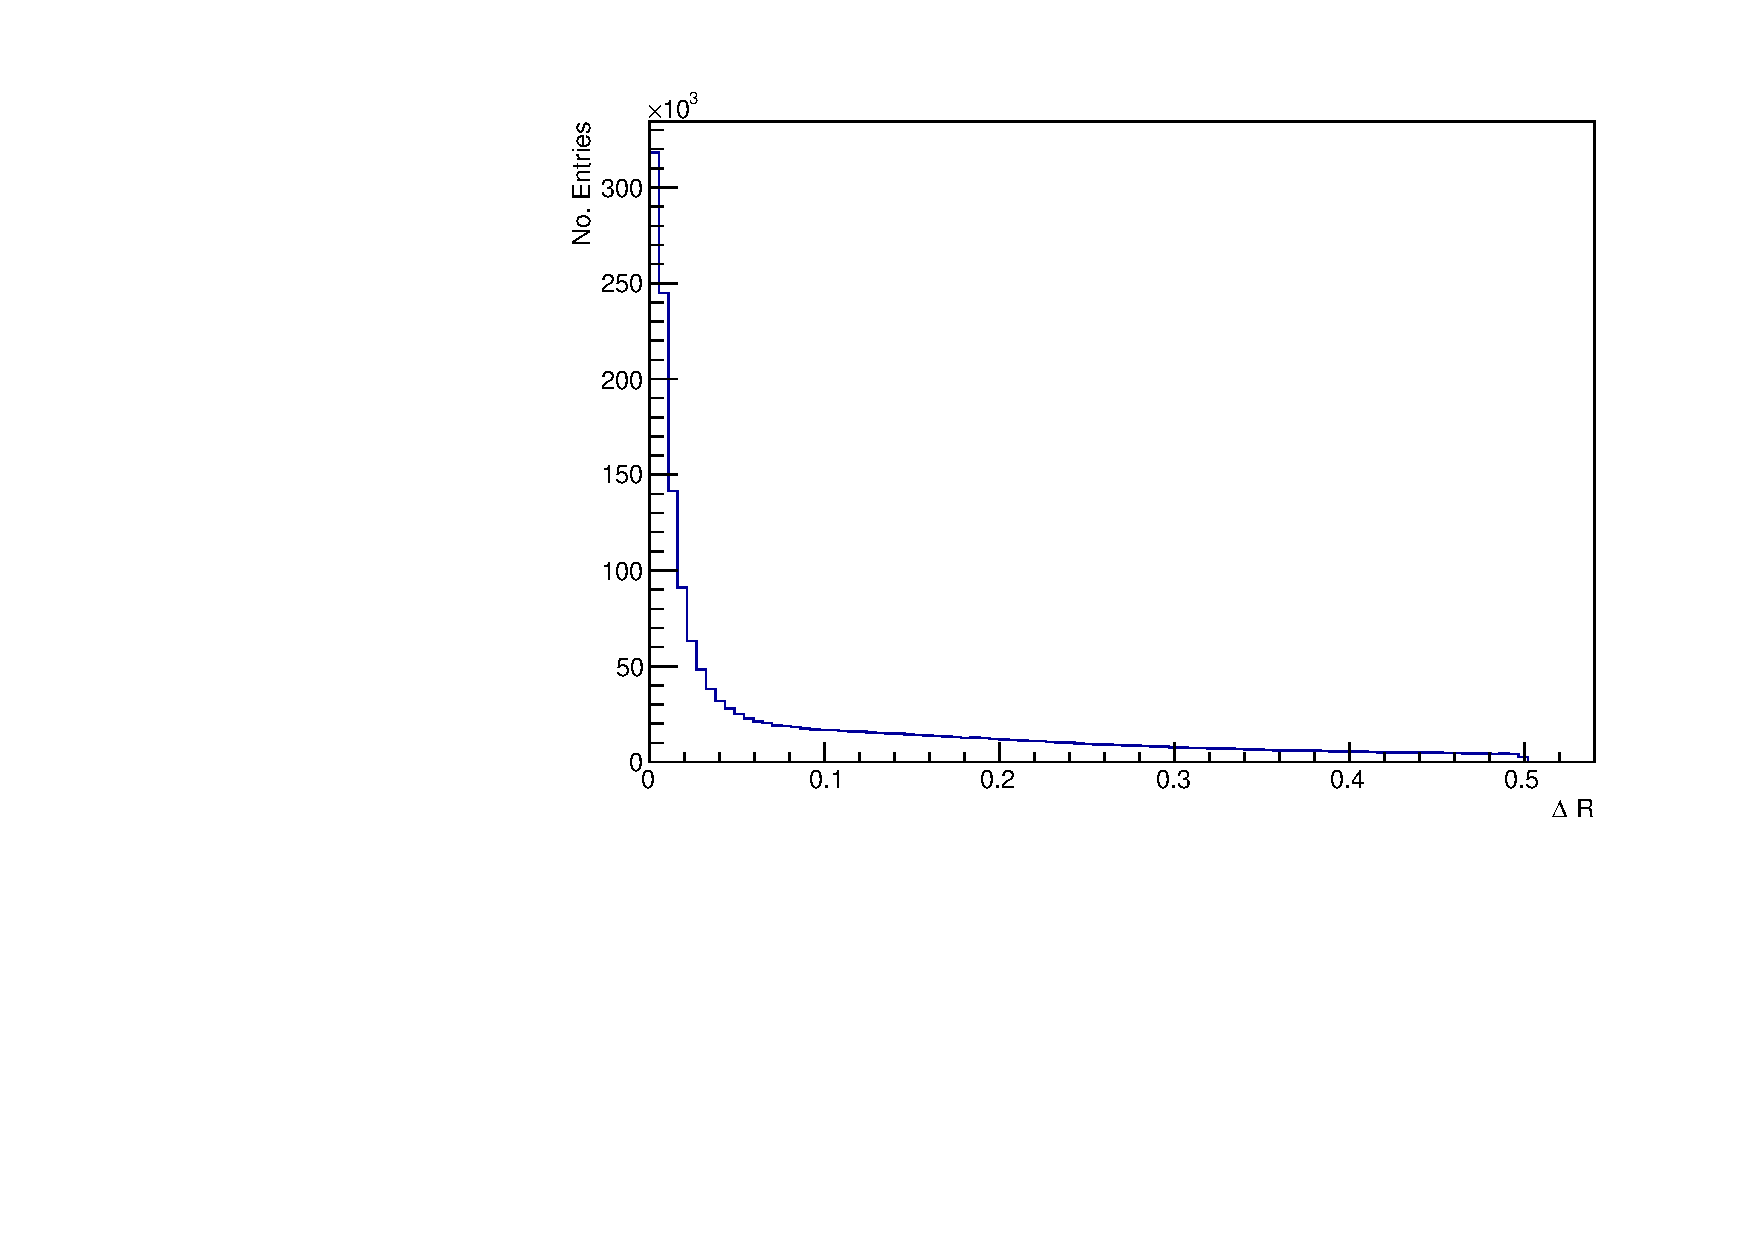
\includegraphics[width=0.8\textwidth]{delR.pdf}
\end{frame}
\end{document}
